\section{Transport}
  \begin{frame}
    \frametitle{Aims}
      \begin{itemize}
        \item Interface session layer,
        \item Reliable end-to-end communication,
        \item Order and reassemble received packets (if needed),
        \item Flow control,
        \item Congestion avoidance (if supported by protocol),
        \item Multiplexing
      \end{itemize}
  \end{frame}

  \begin{frame}
    \frametitle{Application identification}
    \begin{block}{Socket address}
      \begin{itemize}
        \item Node identification is made by IP address,
        \item Application identification is made by node identification...
        \item ... and a port. Number between 0 and 65535. (1-1024: root privilege)
        \item \begin{center} ip.ad.dr.ess:port \end{center}
      \end{itemize}
    \end{block}
  \end{frame}

  \begin{frame}
    \begin{figure}
      \centering
      \begin{tabular}{l|c}
        Port  & Protocol \\ \hline
        21    & FTP \\ \hline
        22    & SSH \\ \hline
        23    & Telnet \\ \hline
        25    & SMTP \\ \hline
        80    & HTTP \\ \hline
        443   & HTTPS \\ \hline
        465   & SMTPS \\ \hline
        631   & IPP \\ \hline
        1194  & OpenVPN \\ \hline
        3128, 8080 & Web Proxy \\ \hline
        9418  & git \\ \hline
        23399 & Skype \\ \hline
      \end{tabular}
      \caption{Default port for well known protocol}
      \label{fig:def-port}
    \end{figure}
  \end{frame}

  \begin{frame}
    \frametitle{TCP header}
    \begin{figure}[p]
        \centering
        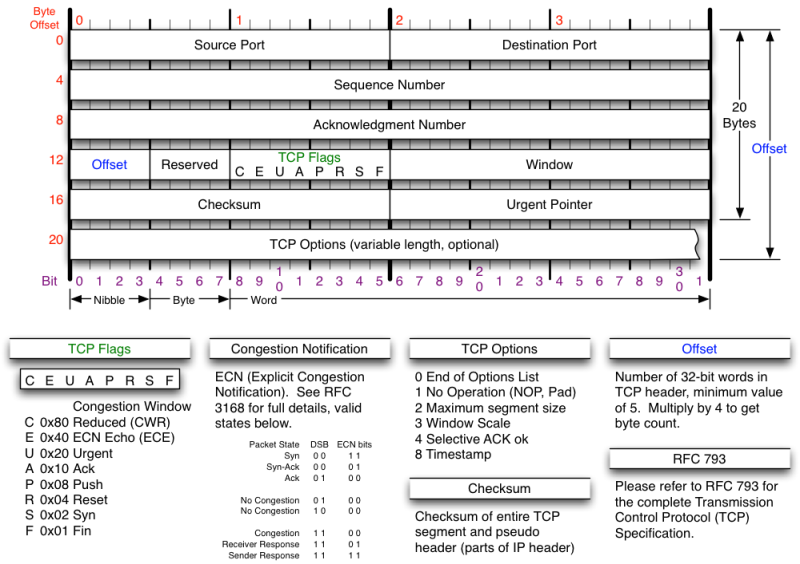
\includegraphics[height=6cm]{./imgs/tcp-hdr.png}
        \caption{\color{blue}\href{http://nmap.org/book/tcpip-ref.html}{nmap.org: TCP header}}
      \label{fig:tcp-header}
    \end{figure}
  \end{frame}

  \begin{frame}
    \frametitle{UDP header}
    \begin{figure}[p]
        \centering
        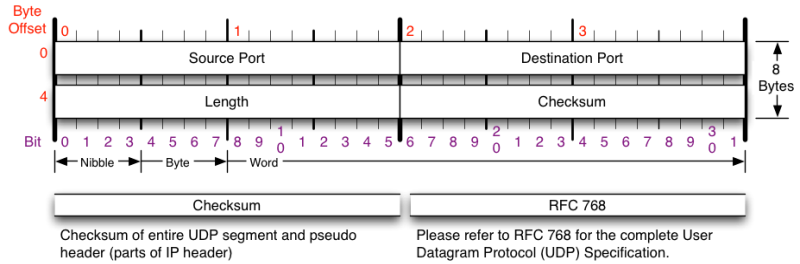
\includegraphics[height=3.5cm]{./imgs/udp-hdr.png}
        \caption{\color{blue}\href{http://nmap.org/book/tcpip-ref.html}{nmap.org: UDP header}}
      \label{fig:udp-header}
    \end{figure}
  \end{frame}

  \begin{frame}
    \frametitle{Socket Primitives (TCP)}
    \begin{figure}
      \centering
      \resizebox{10cm}{!} {
        \begin{tabular}{r|l|l}
          Order & Primitive & Meaning \\ \hline
          1     & SOCKET    & Creates a new communication endpoint \\ \hline
          2     & BIND      & Links local IP address to the socket \\ \hline
          3     & LISTEN    & Signs up for incoming connections \\ \hline
          4     & ACCEPT    & Blocking call till a connection attempt occurs \\ \hline
          -     & CONNECT   & \textbf{Tries} to connect to another communication endpoint \\ \hline
          -     & SEND      & Sends data through the established connection \\ \hline
          -     & RECEIVE   & Receives data through the established connection \\ \hline
          last  & CLOSE     & Releases the connection \\ \hline
        \end{tabular}
      }
      \caption{TCP primitives}
      \label{fig:primitives}
    \end{figure}
    A socket does not have an IP address until it is bound, just an allocation in the transport entity. A server must listen before any client can connect.
  \end{frame}

  \begin{frame}
    \frametitle{What are these  ?}
      \begin{itemize}
        \item \textbf{Frame}: Physical layer representation
        \item \textbf{Datagram}: UDP\footnote{User \textbf{Datagram} Protocol} or IP packet (IP datagram, UDP datagram)
        \item \textbf{Segment}: TCP data unit
        \item \textbf{PDU}: Protocol Data Unit, generic term.
        \item \textbf{Fragment}: Any data unit \textbf{fragmented}
      \end{itemize}
    %TODO: Frame, Packet, PDU, Datagram, Fragment, + header
  \end{frame}
